%!TEX root = ../PatilM-[RnD-MT]Report.tex

\chapter{Experimental Evaluation}

\paragraph{} The primary goal of this chapter is to provide vital information regarding the empirical evaluation that was carried out to validate the proposed approach. The following sections will discuss the practical use cases for the developed system and give a brief overview of the general test setup of the performed experiments before diving into the details of the experiments themselves. A logical analysis of the obtained results will be performed to conclude the chapter.

\section{Use Cases}
\paragraph{} The main aim of this project is to evaluate the efficiency paradigm of qualitative spatial representations for navigation in mobile robots, especially in closed indoor spaces where quantitative representations of the physical space are considered excessive and unnecessary. Therefore keeping in mind these preconditions we define the following possible use cases.

\subsubsection*{Use case: Navigating in a corridor environment} 
\paragraph{} A mobile robot is tasked with navigating from point `A' to point `B' in a corridor environment such that it should avoid collision with the walls and any other static or dynamic obstacles if they exist in its path. Furthermore the robot's movement should be such that it avoids any sudden motions that may seem unsafe or unintuitive to an human agent who might interact with the robot. Also chiefly, the robot must achieve this path traversal in a manner that is as efficient as possible ,while dealing with imprecise information about the environment or in extreme cases lack of complete information about the environment. 

\subsubsection*{Resulting Requirements}
\paragraph{} Ideally it is desired that any new functionality that is being implemented must be highly generalizable, but keeping in mind the given problem it is unrealistic to expect a `one size fits all' implementation that works impeccably for all imaginable situations without any restrictions or compromises. Hence a list of requirements resulting from the problem statement and the above described use case is presented below:

\begin{itemize}
	\item The starting position should be irrelevant when navigating the corridor.
	
	\item The detection of the markers or features should be robust with respect to a reasonable speed of the robot.
	
	\item The number of markers or features should not adversely affect the robot's behavior. 
	
	\item The camera used should have a reasonable field of view so that it can see both the walls and their respective features at any given point of time.
	
	\item The camera should be able to capture the features reasonably well, given reasonable lighting conditions.
	
	\item The motion profile of the robot should be a smooth and not disruptive. 
	
	\item It should be able to navigate any corridor irrespective of its size or the color of its walls.
\end{itemize}

\section{Data collection}
\paragraph{}During the development stage of the algorithm it was tested continuously against a set of collected data that served as a simulation for corresponding real world situations. This method served as a good test to ensure robustness of the individual software components as well as the entire system once it was combined together. The data was collected by manually driving around the robot in a corridor and recording the output of the camera video stream(RGB) after markers had been attached to the walls of the corridor. This simulated data served as a backbone for understanding some of the constraints of the developed algorithm such as the minimum number of markers required, the field of view of the camera, the position of the camera, the velocity of the robot and the orientation of the robot to ensure that both the walls and their respective markers are visible. The collected data simulated conditions such as, 
\begin{itemize}
	\item The robot moving along the center of the corridor.
	\item The robot moving along the left/right wall.
	\item The robot moving diagonally across the corridor.
	\item The robot following a zig-zag pattern along the corridor.
\end{itemize} 
\paragraph{} In all these collected videos a set of two markers was placed on the opposing walls such that both the markers lie on the same axis that is perpendicular to the walls, also the markers were placed at equidistant intervals.
\section{General Test Setup}
\paragraph{} The testing of the developed algorithm was carried out in a two step manner wherein during the first step we evaluated the performance of the two implemented calculi for the task of corridor navigation. The performance is evaluated based on three criteria, the effect of the starting positions, the effect of the marker positions and the number of markers. The evaluation was judged based on the number of possible control paradigms that ensued in a crash with either of the walls. This led to the selection of the calculi with the least number of crashes, the selected calculi was then compared against the existing map based navigation approach which uses quantitative spatial representations and has been implemented on the applied robot platform by the `b-it bots' team. This comparison yields a evaluation of the efficiency paradigms for both the approaches.

\paragraph{} A general setup of the performed experiments is presented below, with the specifics of each experiment discussed in a later section.

	\begin{figure}[h!]%
		\centering
		\subfloat[Experimental setup from the robot's point of view]{{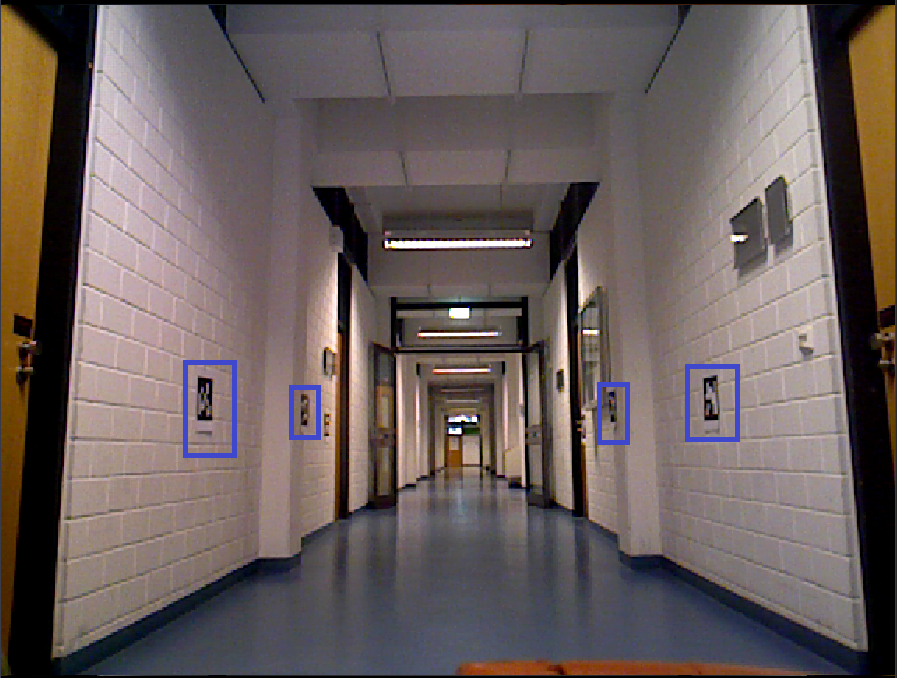
\includegraphics[width=6cm]{images/even_mark} }}%
		\qquad
		\subfloat[Experimental setup from a third person point of view]{{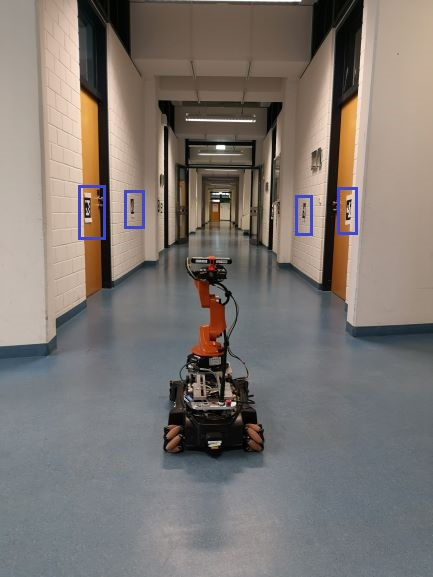
\includegraphics[width=6cm]{images/start} }}%
		\caption{Experimental setup with two sets of markers (indicated using blue boxes) placed along a common perpendicular axis on opposite walls.}%
		\label{fig:point of view}%
	\end{figure}

\subsubsection*{Experiment Variables:}
\begin{itemize}
	\item Initial position and orientation of the robot.
	\item Field of View of the camera.
	\item Lighting conditions of the corridor.
	\item Initial Position of the camera.
	\item Position of the markers relative to the fixed camera position.
	\item Position of the markers relative to each other.
	\item Battery voltage.
	\item Range of the wireless network.
\end{itemize}

\subsubsection*{Software Requirements:}
\begin{itemize}
\item ROS Kinetic
\item Python 2.7 or higher
\item Qsr\_lib package
\item Qsr\_nav package
\item Mir\_bringup package 
\item Mir\_moveit\_youbot\_brsu\_4 package 
\item Moveit\_commander package 
\end{itemize}

\subsubsection*{Hardware Requirements:}
\begin{itemize}
	\item Kuka Youbot
	\item PC capable of runnning ROS
	\item Remote joystick 
	\item Power supply 
	\item Aruco markers
	\item Asus Xtion Pro camera
\end{itemize}

 

\section{Experiments}

\paragraph{}The following section presents the set of experiments that were conducted and evaluated to decide upon a qualitative calculi that was optimal for the task of navigating the corridor.

\paragraph{Note:}When performing the experiments the most common issue faced was the quick discharge of the battery and the loss of communication between the modules and the remote computer.
 
\subsection{Experiments for QTCB calculi}
\subsubsection{Testing the navigational capabilities of the QTCB calculus in a indoor corridor environment} 
\paragraph{}The individual experiments and their respective analysis have been presented in a tabular format in the figures 5.1, 5.2 and 5.3.

\begin{sidewaysfigure}[h!]
	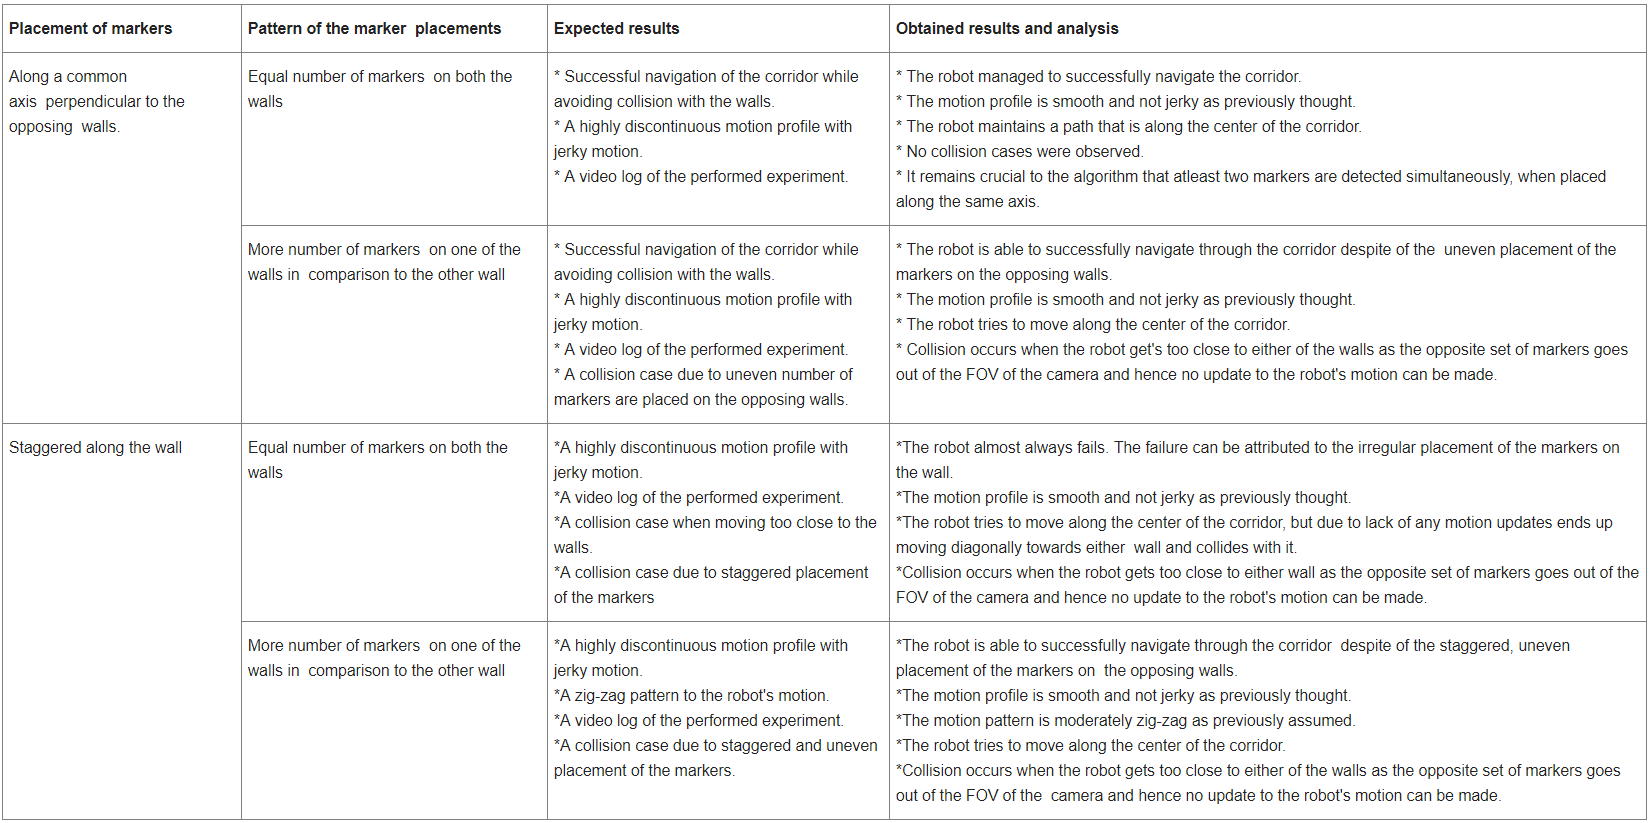
\includegraphics[scale = 0.6]{images/center}
	\caption{Table of conducted experiments for $QTC_B$ and their respective analysis for a starting position that is along the center of the corridor.}
	\label{fig:center}
\end{sidewaysfigure}


\begin{sidewaysfigure}[h!]
	\includegraphics[scale = 0.6]{"images/right table"}
	\caption{Table of conducted experiments for $QTC_B$ and their respective analysis for a starting position that is along the right wall of the corridor.}
	\label{fig:right-table}
\end{sidewaysfigure}


\begin{sidewaysfigure}[h!]
	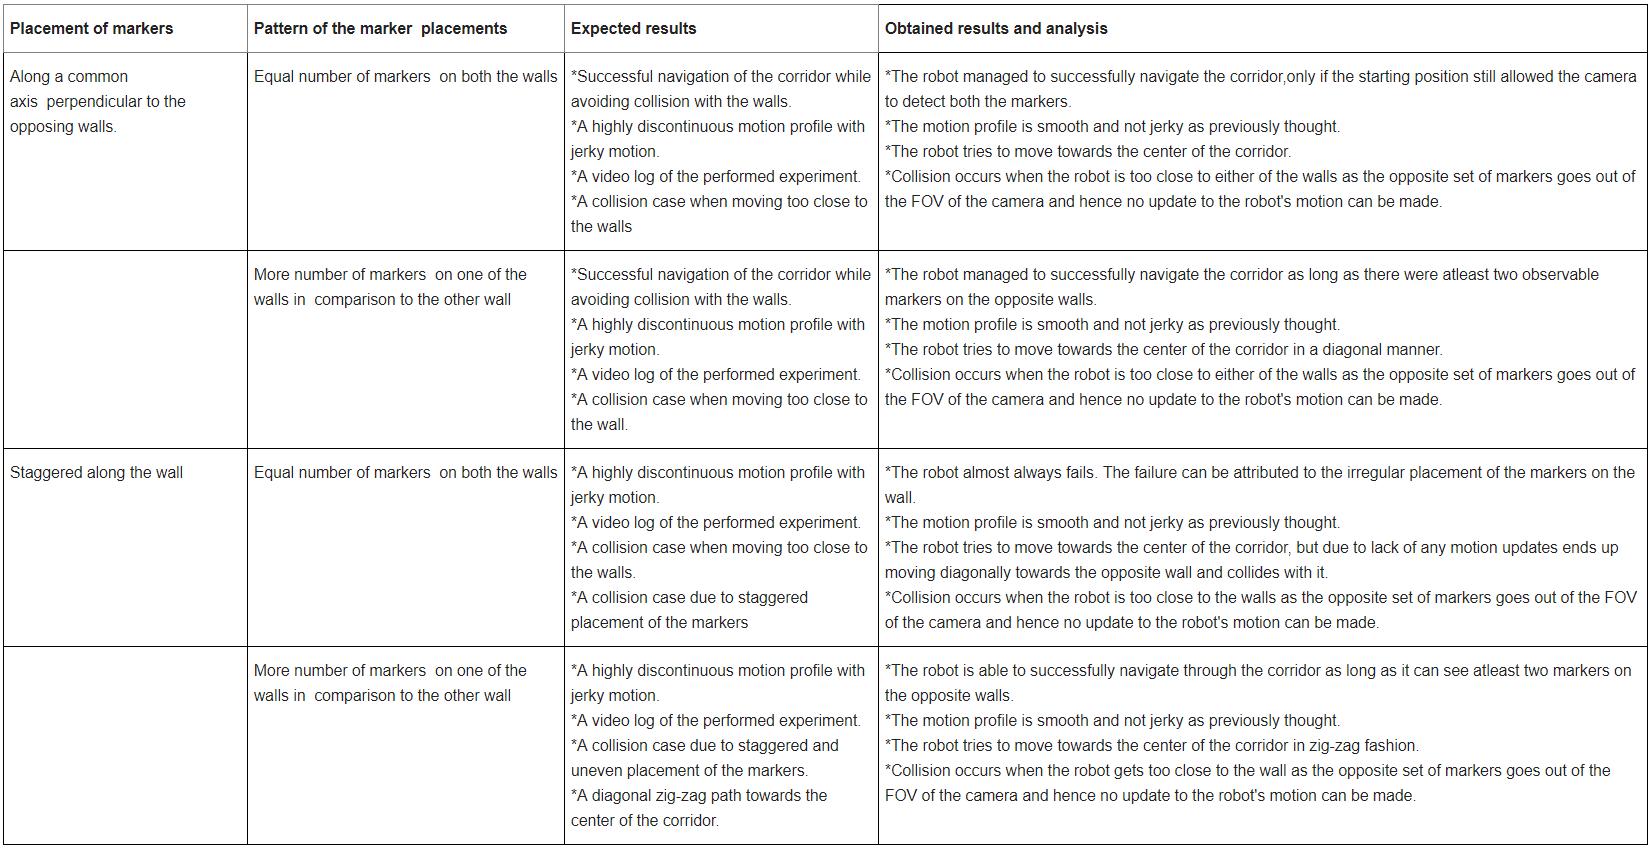
\includegraphics[scale = 0.6]{images/left_table}
	\caption{Table of conducted experiments for $QTC_B$ and their respective analysis for a starting position that is along the left wall of the corridor.}
	\label{fig:left-table}
\end{sidewaysfigure}

\subsubsection*{Evaluation} From the experiment tables presented in the following figures(5.1,5.2,5.3) it is clear to see that the main reason for failure of the QTCB calculus is the limited FOV of the camera used. Also the tabular structure makes it clear to understand that the the algorithm is robust enough to function with an arbitrary number and placement of the markers with the only failure occurring when it cannot detect atleast two markers placed on opposite walls. Additionally out of all the test scenarios the only clear failure(irrespective of starting position) of the algorithm was when the markers were placed in a staggered manner along the walls, this was also due to the fact that the camera's FOV is limited and prevented it from detecting both the markers at all instances of time. All the experiments were carried out such that they travel from point `A' to `B' and back from `B' to `A' this was done to ensure that the detection component isn't favorable to any one side or travel and is robust enough to function even if the markers on the opposing walls were interchanged. Out of a set of 12 experiments conducted the QTCB representation was able to perform collision free navigation in all but 1 set of experiments giving it a success rate of 83.3 percent.

\subsection{Experiments for ARGD calculi}
\subsubsection{Testing the navigational capabilities of the ARGD calculus in a indoor corridor environment} 
\paragraph{}The individual experiments and their respective analysis have been presented in a tabular format in the figures 5.4, 5.5 and 5.6. For the ARGD calculus the distance thresholds used for discretizing continuous space are an additional experiment variable that affects the representation of physical space.

\begin{sidewaysfigure}[h!]
	\centering
	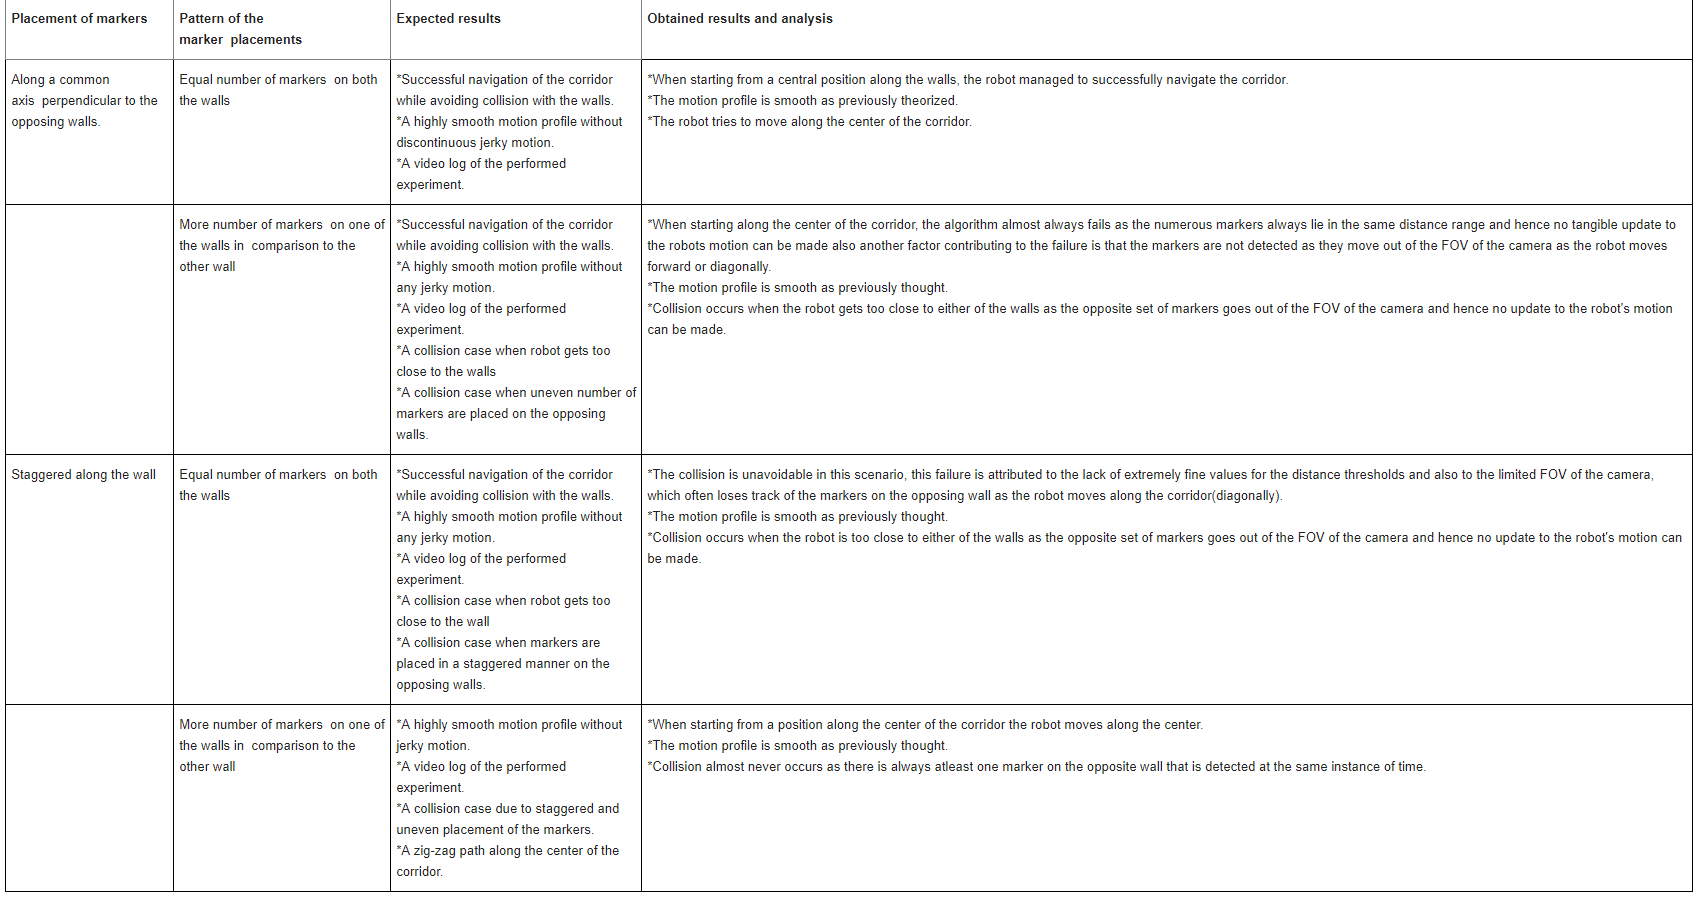
\includegraphics[scale = 0.6]{images/argd_center}
	\caption{Table of conducted experiments for $ARGD$ and their respective analysis for a starting position that is along the center of the corridor.}
	\label{fig:argdcenter}
\end{sidewaysfigure}


\begin{sidewaysfigure}[h!]
	\centering
	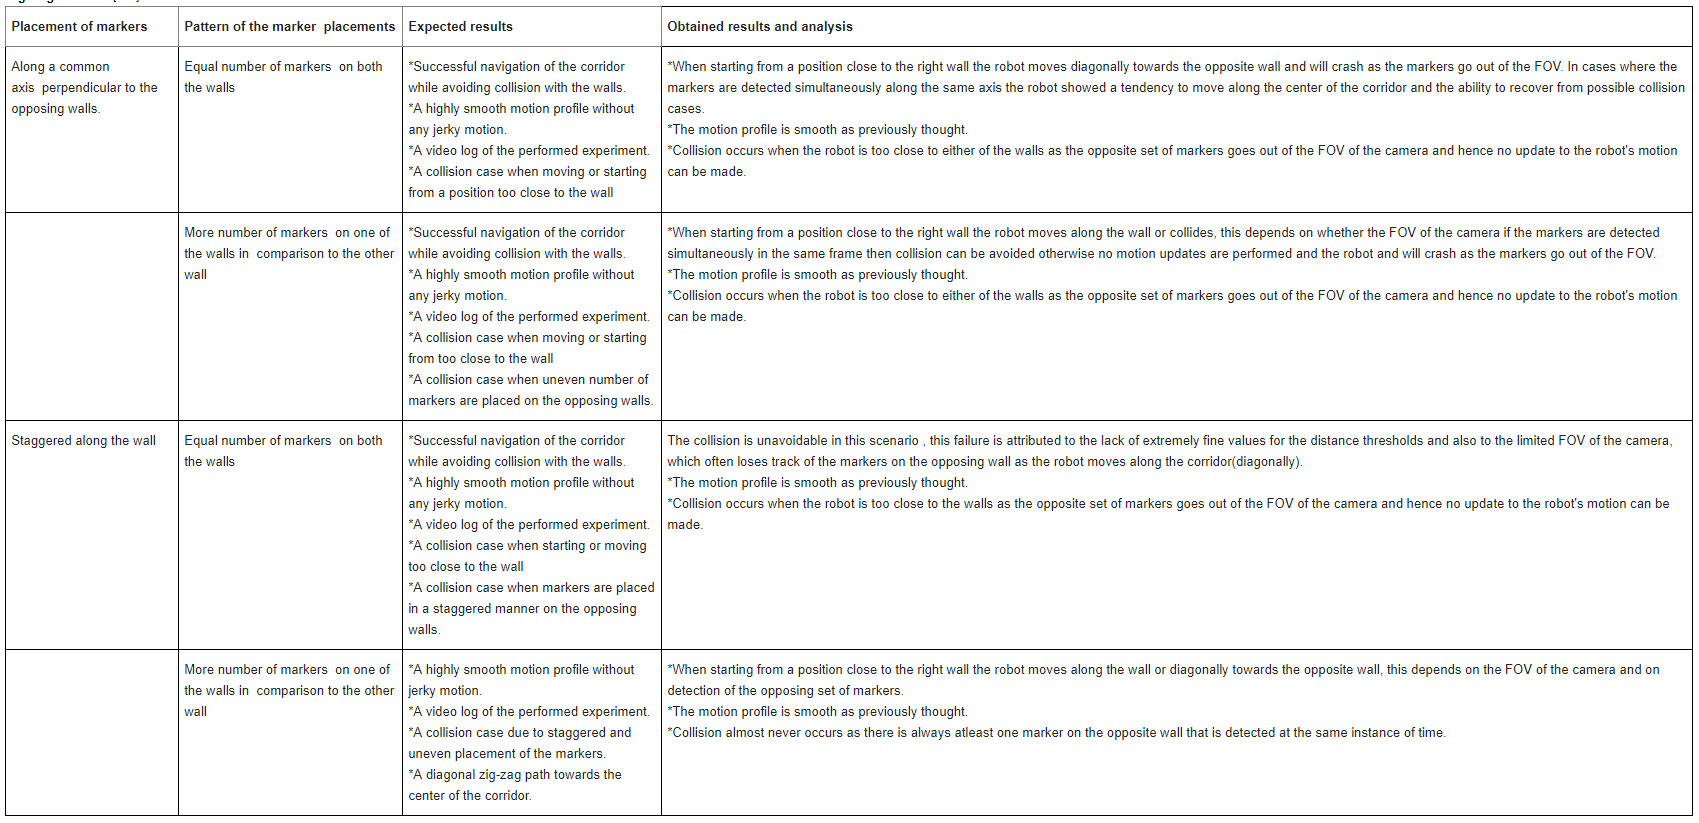
\includegraphics[scale = 0.6]{images/argd_right}
	\caption{Table of conducted experiments for $ARGD$ and their respective analysis for a starting position that is along the right wall of the corridor.}
	\label{fig:argdright}
\end{sidewaysfigure}

\begin{sidewaysfigure}[h!]
	\centering
	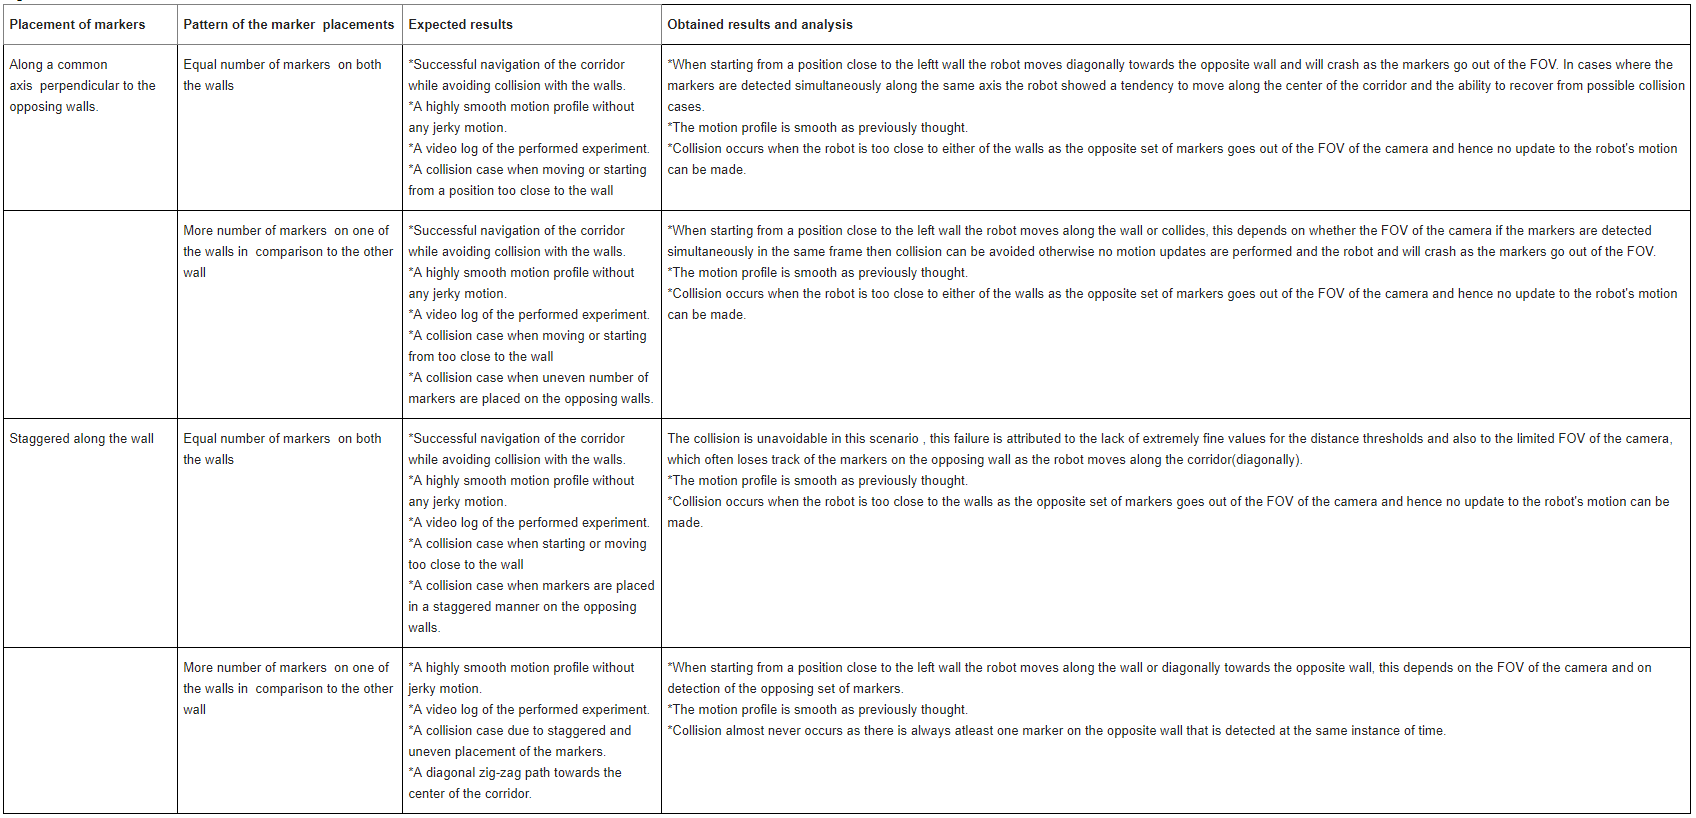
\includegraphics[scale = 0.6]{images/argd_left}
	\caption{Table of conducted experiments for $ARGD$ and their respective analysis for a starting position that is along the left wall of the corridor.}
	\label{fig:argdleft}
\end{sidewaysfigure}
 
\subsubsection*{Evaluation} From the experiment tables presented in the following figures(5.4, 5.5, 5.6) it is clear to see that there are two main reasons for failure of the ARGD calculus the first is the limited FOV of the camera used and the second is the inability of the calculi to distinguish between two objects that lie in the same distance thresholds, due to this the number of failure cases is higher for the ARGD when compared to the $QTC_B$. Also the tabular structure makes it clear to understand that the algorithm isn't robust enough to function with any arbitrary number and placement of the markers with collisions(with respect to the walls) occurring regularly in nearly all the test cases.One of the clearest cases of failure was when the markers were placed in a staggered manner along the walls, this was a clear illustration of the ARGD being an insufficient calculi when it comes to dealing with mobile objects, with the need for fine distinctions between the objects lying in the same distance threshold being clearly highlighted in this case. All the experiments were carried out such that they travel from point `A' to `B' and back from `B' to `A' this was done to ensure that the detection component isn't favorable to any one side or travel. Out of a set of 12 experiments conducted the ARGD representation was able to perform collision free navigation in all but 4 sets of experiments giving it a success rate of 66.6 percent.

\subsection{Common Observations}
\begin{itemize}
	\item All the movements observed during the experiments are gradual and there is no sudden change to the robot's velocity or speed.
	\item The algorithm can be made more robust if the $ARGD$ and the $QTC_B$ calculus can be combined, this is possible with the current implementation but is complicated as the number of rulesets would increase exponentially with respect to the objects in consideration.
	\item In the current setup the algorithm is inherently dependent on the perception module(it reacts to what it sees, currently we look for markers or features on the wall, if this changes to looking for features on the ceiling or floor then the representation and control modules will also have to be changed accordingly) and any changes to this module would likely warrant changes to the entire setup especially in the case of the distance based $ARGD$ calculus, the $QTC_B$ calculus on the other hand would only require that the number of objects in consideration be changed to the desired number.
	\item The current setup uses small velocity values to control the robot with the maximum value being 0.1 m/s and the lowest being 0.02 m/s.
	\item Improvements to the current algorithm can also be made using different setup of the cameras where two cameras facing the opposite wall may be used.
	\item The current implementation also uses a time based filter to build relations only when two or more markers are detected simultaneously at similar timesteps, in cases where only a single object is used to build the relation with the robot this filtering must be removed to ensure successful navigation.
	\item Also if more than two objects are to be used when calculating the motion updates then, filtering has to be done to ensure that there is no repetition when building the relations that are consequently used for the decision making process.
\end{itemize}

\subsection{Conclusion} 
\paragraph{} From the above breakdown of the results it is easy to see that the $QTC_B$ calculi outperforms the $ARGD$ calculi when it comes to the task of collision free robot navigation. As discussed above this is attributed to the fact that the distance calculi lacks the tools to distinguish between markers or features that lie in the same distance thresholds, furthermore due to the limited representation capabilities there exist very few instances where a clear distinction between the markers can be made hence resulting in a fewer number of instances where suitable control commands can be exercised. Beyond this, both the calculi suffered failures due to the limited FOV of the camera as it prevented the detection of the markers lying on the opposing walls whenever the robot moved close to either of the walls(it remains crucial to the algorithm that atleast two markers are detected simultaneously, when placed along the same axis or otherwise). To compliment the validity of the results it is worth mentioning that the $ARGD$ calculus works on abstractions of spatial distances and was developed for representing and reasoning about static objects whereas the $QTC_B$ calculi works on abstractions of relative trajectories between two objects and was developed representing and reasoning about mobile objects, hence it is obvious that it should perform better than the $ARGD$ calculus for the given task. Thus based on this empirical evidence we select the $QTC_B$ calculi to compare and evaluate the efficiency paradigms against a quantitative map based representation.


\section{Evaluation of the efficiency of qualitative representations}
\paragraph{}Based on the above validation efficiency of the $QTC_B$ calculi was compared against the map based navigation technique that utilized quantitative spatial representations, on the task of navigating from point `A' to `B' in the corridor. The starting positions were kept approximately same for the purpose of this testing and the average velocity values were ensured to be same. Furthermore since we would like to evaluate the battery consumption a fully charged battery was used during the tests for each representation. The experiment was repeated thrice for each of the representations so as to obtain any variance in the values and ensure accurate resulting values. For the purpose of this evaluation the $QTC_B$ experiment was setup so that the markers always lay on the same perpendicular axis to the wall and the number of markers on both the walls was the same, the starting position was always along the center of the corridor.

\newpage

\begin{table}[h!]
	\begin{adjustwidth}{-1cm}{}
	\begin{tabular}{|p{2cm}|p{2cm}|p{2cm}|p{2.5cm}|p{2cm}|p{2cm}|p{2.5cm}|}
		\hline
		Experiment number & Starting Battery Voltage (volts) & Ending Battery Voltage (volts) & Average Battery Voltage (volts) & Duration of the Experiment(in seconds) & Total Velocity commands issued & Velocity commands per second (messages/second) \\ \hline
		1 & 12 & 12 & 12 & 39.4 & 309 & 7.8 \\ \hline
		2 & 12 & 12 & 12 & 41.7 & 321 & 7.6 \\ \hline
		3 & 12 & 12 & 12 & 36.5 & 317 & 8.6 \\ \hline
		&  &  & Gross Avg. : 12 &  &  & Gross Avg. : 8.0 \\ \hline
	\end{tabular}
	\caption{Computational and power consumption statistics for quantitative map based navigation.}
	\label{map based table}
	\end{adjustwidth}
\end{table}

\begin{table}[h!]
	\begin{adjustwidth}{-1cm}{}
	\begin{tabular}{|p{2cm}|p{2cm}|p{2cm}|p{2.5cm}|p{2cm}|p{2cm}|p{2.5cm}|}
		\hline
		Experiment number & Starting Battery Voltage (volts) & Ending Battery Voltage (volts) & Average Battery Voltage (volts) & Duration of the Experiment(in seconds) & Total Velocity commands issued & Velocity commands per second (messages/second) \\ \hline
		1 & 11 & 11 & 11 & 103 & 1177 & 11.4 \\ \hline
		2 & 11 & 11 & 11 & 69 & 751 & 10.8 \\ \hline
		3 & 11 & 11 & 11 & 65 & 1333 & 20.5 \\ \hline
		&  &  & Gross Avg. : 11 &  &  & Gross Avg. : 14.2 \\ \hline
	\end{tabular}
	\caption{Computational and power consumption statistics for the developed qualitative spatial ($QTC_B$) representation based navigation approach.}
	\label{qualitative table}
\end{adjustwidth}
\end{table}
\newpage
\begin{figure}[H]
	\subfloat[Plot showing the robot's general path through the corridor when using the qualitative approach, the bottom left indicate the start point and the top right indicates the end.]{{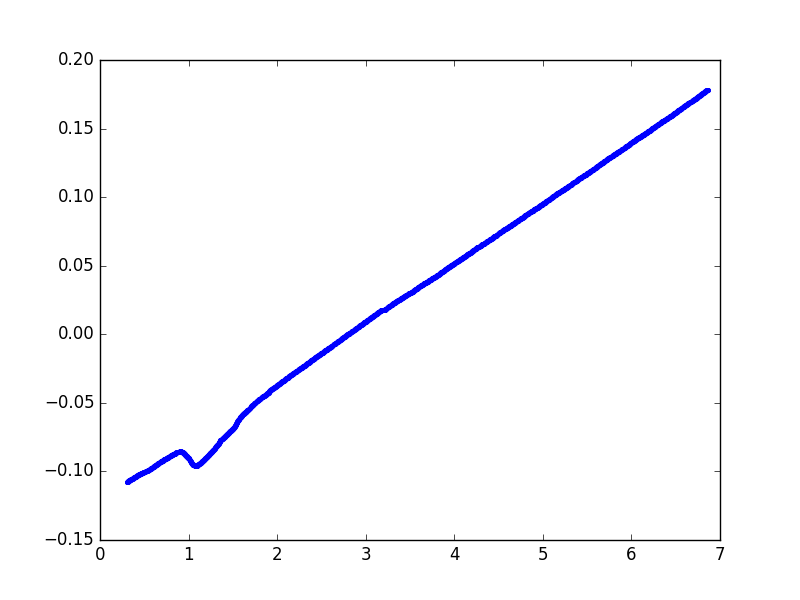
\includegraphics[width=6cm]{images/25_40} }}%
	\qquad
	\subfloat[Plot showing the robot's general path through the corridor when using the quanititative map based approach, the bottom left indicate the start point and the top right indicates the end.]{{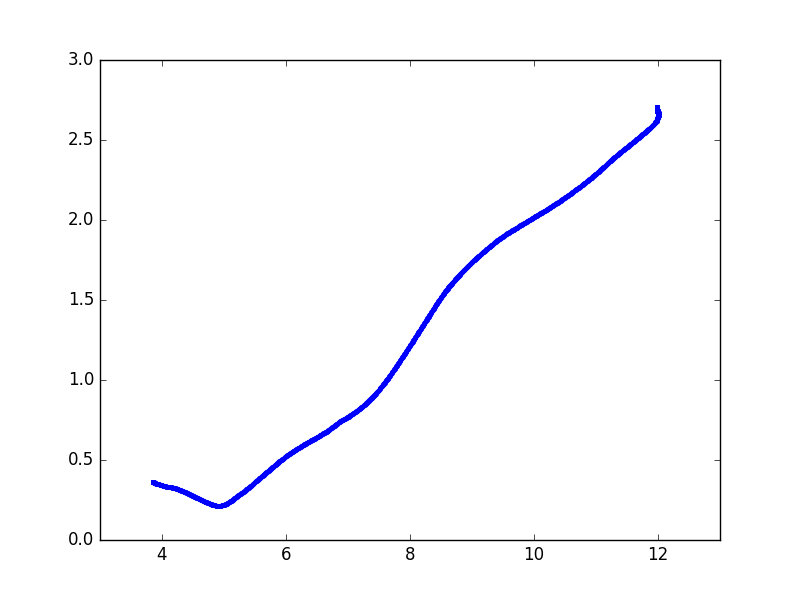
\includegraphics[width=6cm]{images/57_26} }}%
	\caption{Image showing the general path (approximately 7 meters in length) of the robot when using either of the two approaches being compared in section 5.5(the corridor's walls lie along the path, parallel and equidistant to each other)}%
	\label{fig:path}%
\end{figure}

\section{Conclusion}
Due to a lack of decisive data regarding the battery statistics we cannot make any concrete arguments over the power consumption efficiency of the qualitative representations in comparison to the quantitative representations, a better data collection approach that depicts the battery statistics in a much more accurate manner is needed for further examination. Therefore we evaluate the efficiency paradigm from a computational point of view.From a brief glance at the above comparison it is easy to conclude that qualitative representations aren't exactly as efficient as they are made out to be. Yet, the result is not a direct effect of the qualitative representations themselves, but a combination of various other factors that contribute towards the final outcome. For instance, in our implementation we do not discern between two motion updates that are the same for consecutive instances of time, this leads to a large number of duplicate velocity commands issued (hence the large number in table 5.2) which in-turn increases the duration of the recorded bagfile. To give a more comprehensive idea of the effect of accounting for this redundant data we analyzed the data from the third experiment and found out that out of the total 1333 velocity commands issued only 460 were non-duplicated amongst consecutive time steps this effectively translates to 7.07 times that the robot's motion was updated (via the velocity messages) in a single second, thus showing a slight improvement in computational efficiency over the map-based approach. Therefore we establish that the utilization of qualitative representations does provide a slightly better computational efficiency but not enough to conclusively claim that it is more efficient than numerical quantitative representations. On the other hand our implementation of these qualitative approaches still requires additional work to achieve this improvement in efficiency, however small it might be. 

